\subsection{Long-Range Spatio-Temporal Task} \label{synth-benchmark:long}

\looseness-1  Finally, we introduce \emph{long-range spatio-temporal tasks} to evaluate how effectively TGL methods reason across both temporal and spatial dimensions. These tasks extend the delayed cause-and-effect framework by incorporating multi-hop spatial paths alongside temporal dependencies. In this setting, each graph snapshot contains multiple paths originating from a source node \(v_{\mathcal S}\), while a target node \(v_{\mathcal T}\) connects to the endpoints of paths appearing \(\lag\) time steps earlier. We formalize this task as follows:
 
\begin{definition}[Long-Range Spatio-Temporal Task]
\looseness-1 Let \(\lag, d, P \in \mathbb{N}\). The \emph{long-range spatio-temporal task} family $ \mathcal{L}\hspace{-0.035cm}\mathcal{R}_P(\lag,d)$ is defined over dynamic graphs \(\mathcal{G} = G_1, G_2, \dots\), where each snapshot $G_t = (V, E_t)$ has a fixed node set $V = \{v_{\mathcal S}, v_{\mathcal T}, v_1, \dots, v_{N}\}$. The edge set $E_t$ consists of $P$ disjoint paths of length $d$ from the source node $v_{\mathcal S}$ through randomly chosen intermediate nodes. For $t > \lag$, $E_t$ additionally includes $P$ edges from the target node $v_{\mathcal T}$ to the endpoints of the $P$ paths in $G_{t - \lag}$. Formally, for $t > \lag$:
$E_t = \bigcup_{p=1}^P \{(v_{\mathcal S}, u_1^{(t,p)}), (u_1^{(t,p)}, u_2^{(t,p)}),\dots, (u_{d-1}^{(t,p)}, u_d^{(t,p)})\} \cup \\ \{(v_{\mathcal T}, u_d^{(t-\lag,p)})\}$, where the nodes $u^{(t,p)}_{i}$ for $1\leq i\leq d$, $1\leq p \leq P$ are drawn at random in $\{v_1,\dots,v_N\}$~(without replacement).
\end{definition}\label{def:long_range}


Intuitively, we can treat node $v_\mathcal{S}$ as the \textit{progenitor} of some signal that 1) reaches a set of nodes that are spatially separated from $v_\mathcal{S}$ by a distance $d$ and 2) whose effect (connecting the nodes that it reached to node $v_\mathcal{T})$ is additionally delayed by $\lag$ timesteps.
An illustration of a dynamic graph for this task is given in Figure~\ref{fig:longrange}.
%Here, given $P = 3, d = 3$, observe that at $t = 1$, $S$ is connected to 3 paths of length 3. The terminal nodes of these paths, namely $8, 9, 11$ are then connected to target $T$ after a lag of 1. 
We will focus on the effect of the lag $\lag$  and distance $d$ in our experiments and set the number of path $P$ to $3$ in all tasks, which we will simply denote by $\longrange{\lag,d}$.

\begin{figure}
    \centering
    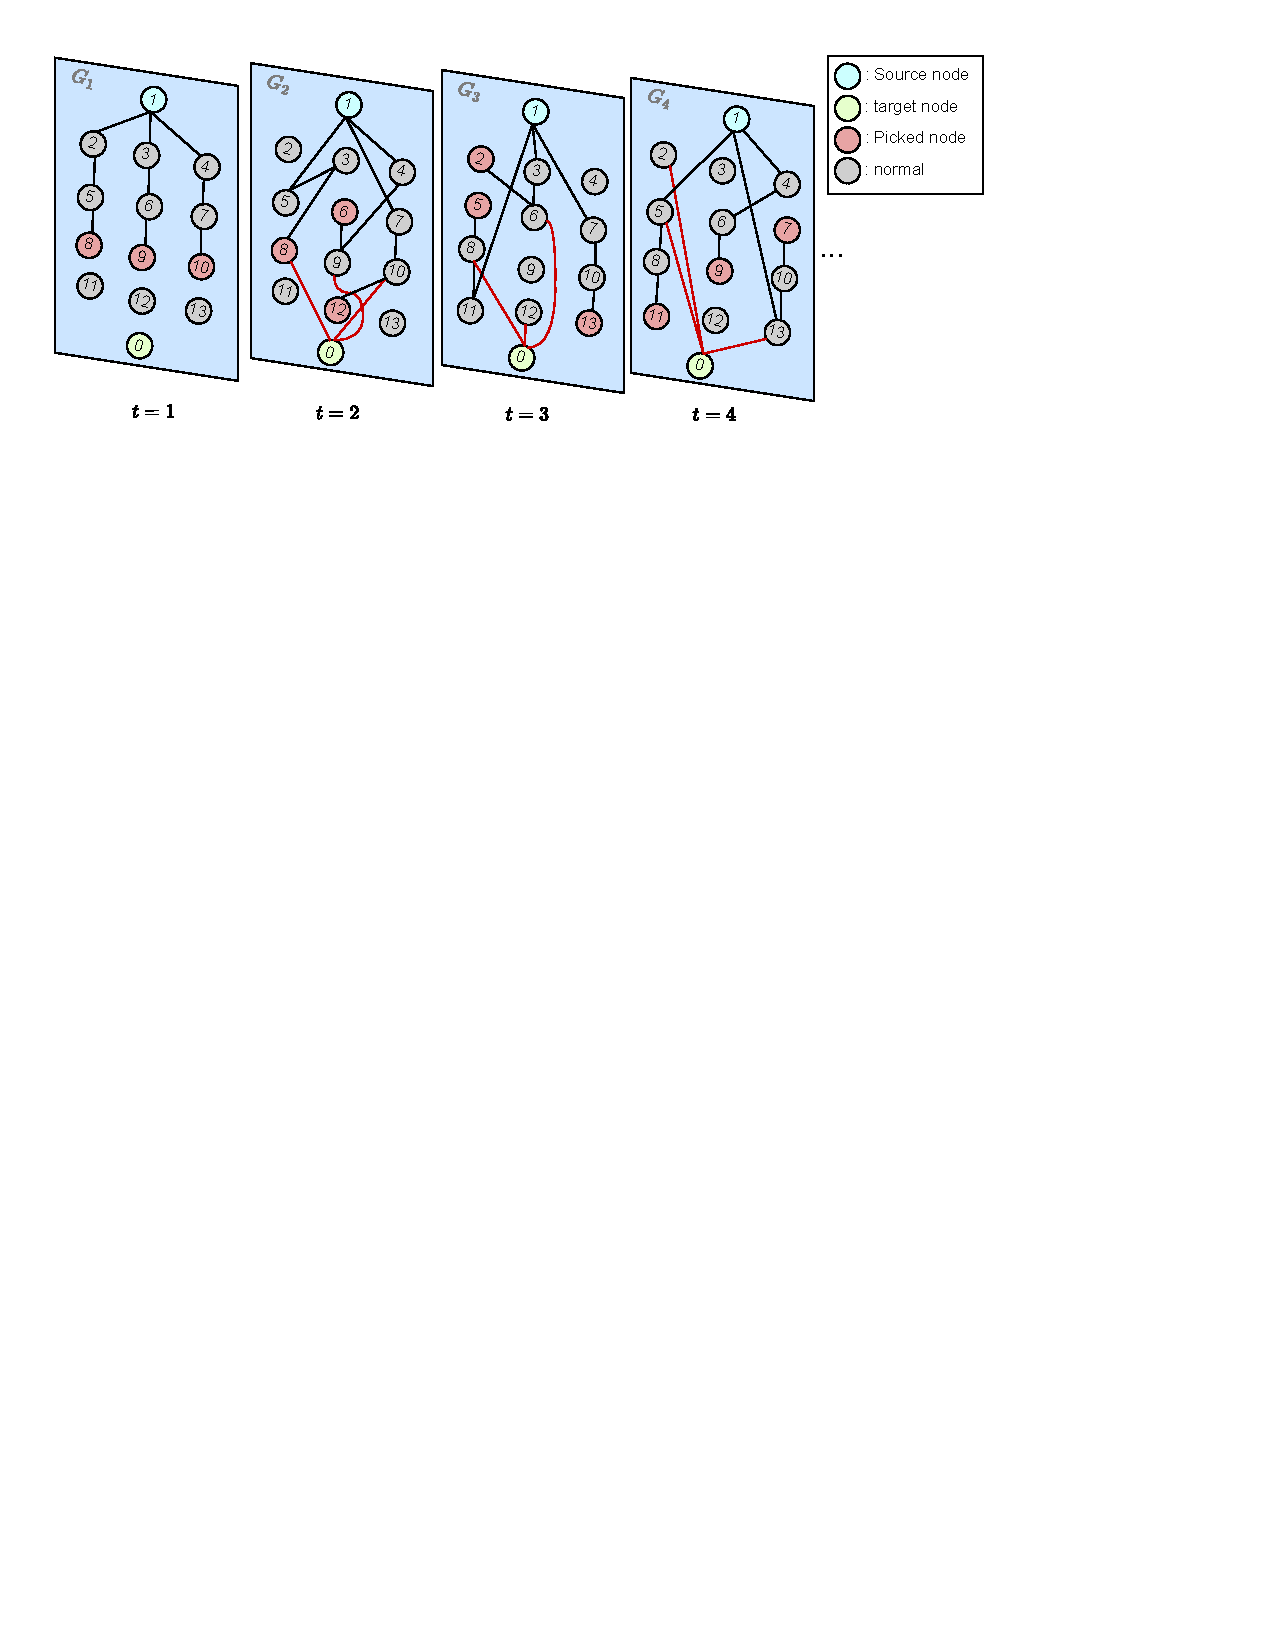
\includegraphics[width=\linewidth, height=11.0em, keepaspectratio]{figs/long_range/fig.pdf}
    \caption{Illustration of a long-range spatio-temporal task $\longrange{\lag,d}$ with    $\ell=1$, $d=3$ and $P=3$.}
    \label{fig:longrange}
\end{figure}


\textbf{Task objectives and implementation.}
Dynamic graphs inherently contain two fundamental distance metrics: temporal (between time steps) and spatial (between nodes). Effective TGL methods must reason across both dimensions simultaneously to capture complex patterns. The \(\longrange{\lag,d}\) task family specifically evaluates this capability by requiring models to track information across both temporal lags and multi-hop spatial paths. The parameter \(\lag\) determines the temporal memory requirement, while \(d\) defines the spatial propagation distance. This dual-parameter design creates a comprehensive benchmark for assessing spatio-temporal reasoning depth in TGL architectures. To systematically evaluate model capabilities, we generate tasks with increasing complexity using distance values $d \in \{1, 2, 4, 8, 16\}$ and temporal lags $\lag \in \{1, 4, 16, 32\}$.


\textbf{Results.} Figure~\ref{fig:plots_long_range} presents $F_1$ scores for top-performing methods and the EdgeBank baseline 
% (complete results in Appendix~\ref{apendix:spatio_temporal_full_methods})
. At small temporal lags, both DTDG approaches and DyGFormer demonstrate strong performance. However, as $\lag$ increases, DTDG methods exhibit sharp performance declines, revealing limitations in recurrent architectures' capacity to maintain long-range temporal memory. DyGFormer's performance deteriorates more gradually but still struggles with extended temporal dependencies. In contrast, TGAT and TGN maintain robust performance even at substantial lags ($\lag=16,32$), highlighting the efficacy of attention-based message passing for complex spatio-temporal reasoning. Nevertheless, all models, even the strongest temporal reasoners, show significant performance degradation when spatial distance exceeds $d=8$, emphasizing the persistent challenge of capturing long-range spatial dependencies in dynamic graphs.



\begin{figure*}[t]
    \centering
    \begin{subfigure}[b]{0.24\textwidth}
        \centering
        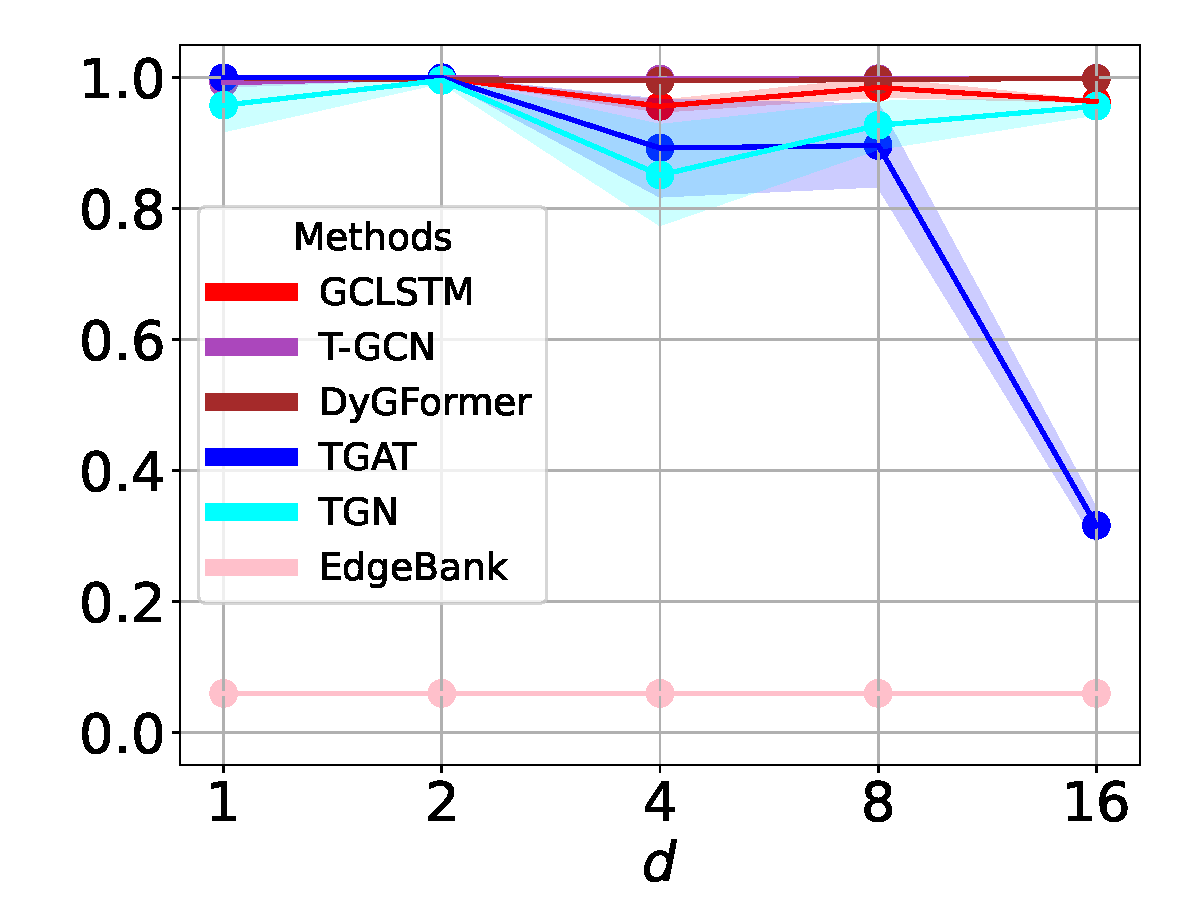
\includegraphics[width=\linewidth]{figs/long_range/fig(10, 10)/(1, d)Best_Test $F_1$.pdf}
        \caption{$(\ell=1, d)$}
        \label{fig:sub_long_range_(1,d)}
    \end{subfigure}
    \begin{subfigure}[b]{0.24\textwidth}
        \centering
        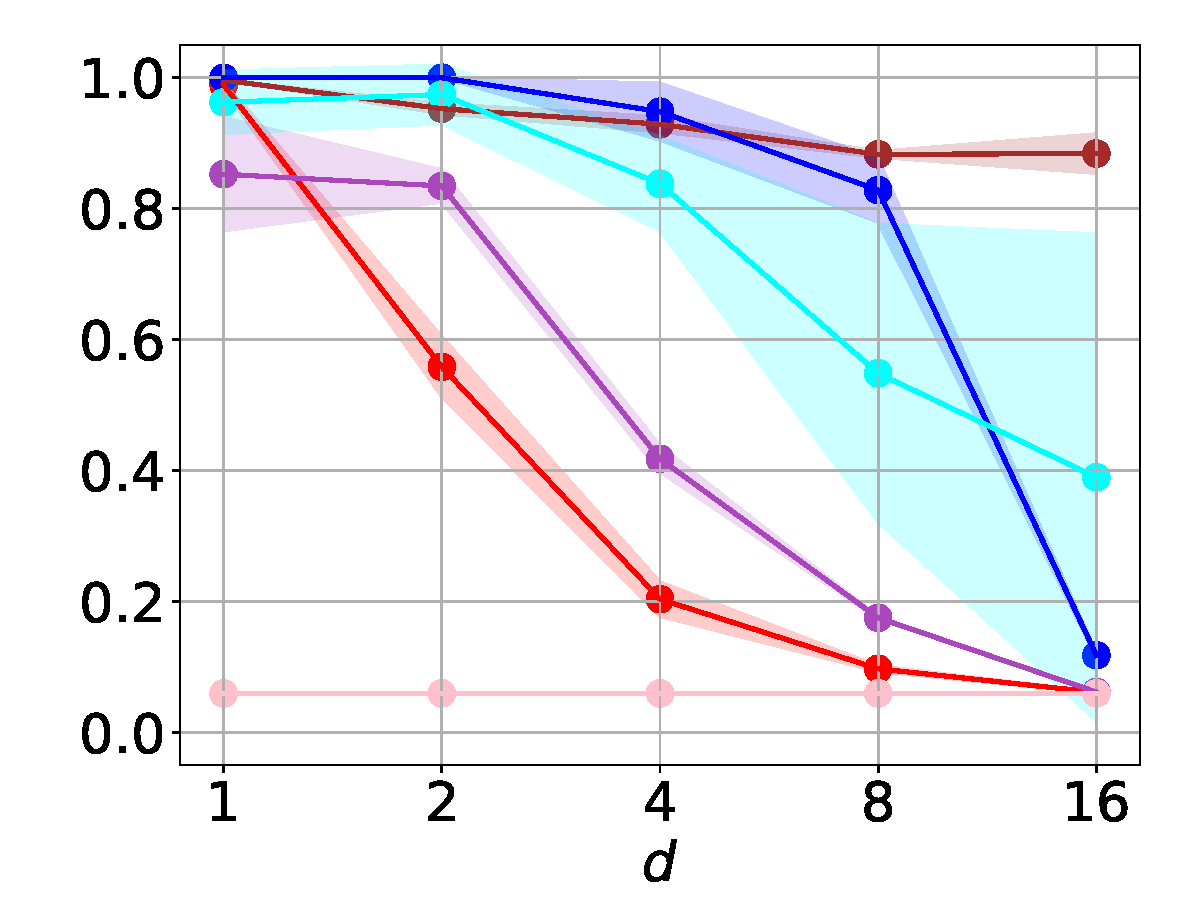
\includegraphics[width=\linewidth]{figs/long_range/fig(10, 10)/(4, d)Best_Test $F_1$.pdf}
        \caption{$(\ell=4, d)$}
        \label{fig:sub_long_range_(4,d)}
    \end{subfigure}
    \centering
    \begin{subfigure}[b]{0.24\textwidth}
        \centering
        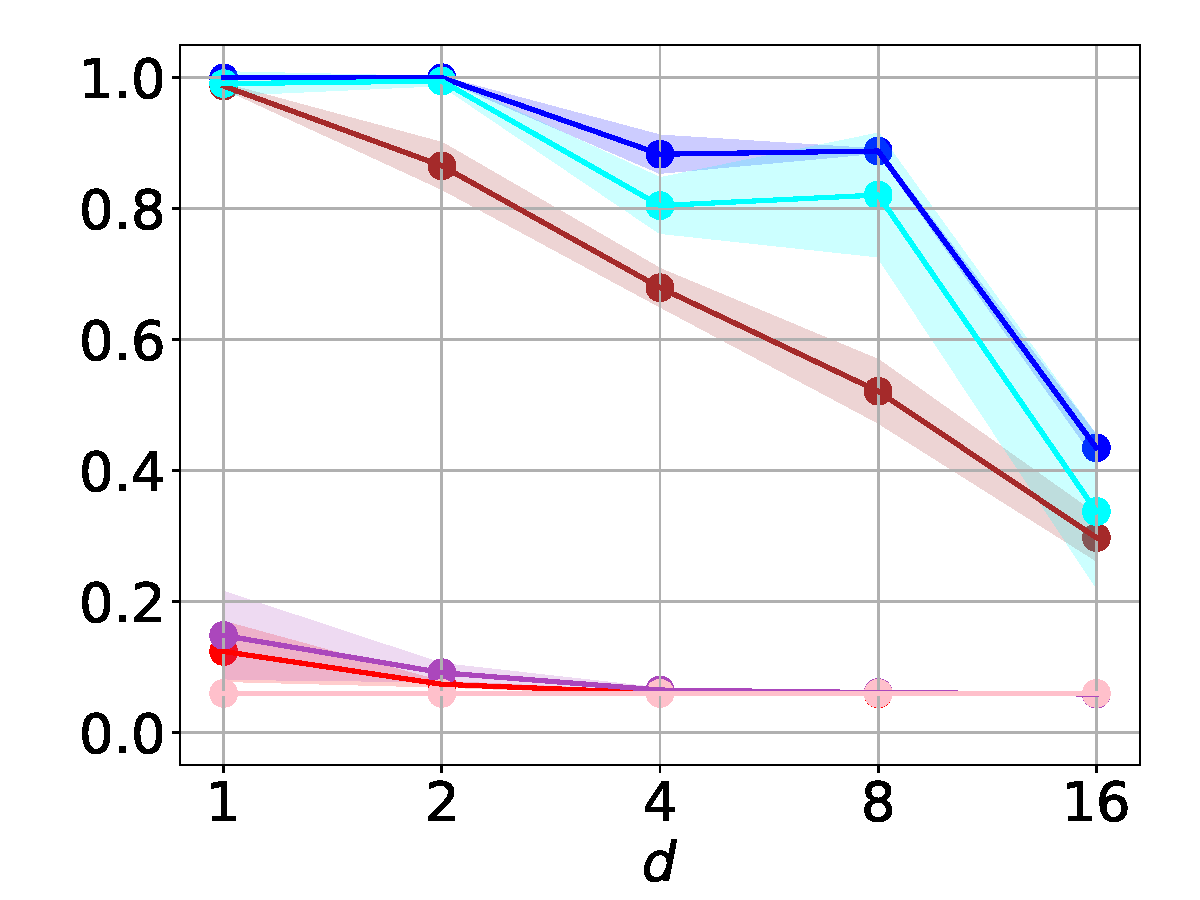
\includegraphics[width=\linewidth]{figs/long_range/fig(10, 10)/(16, d)Best_Test $F_1$.pdf}
        \caption{$(\ell=16, d)$}
        \label{fig:sub_long_range_(16,d)}
    \end{subfigure}
    \begin{subfigure}[b]{0.24\textwidth}
        \centering
        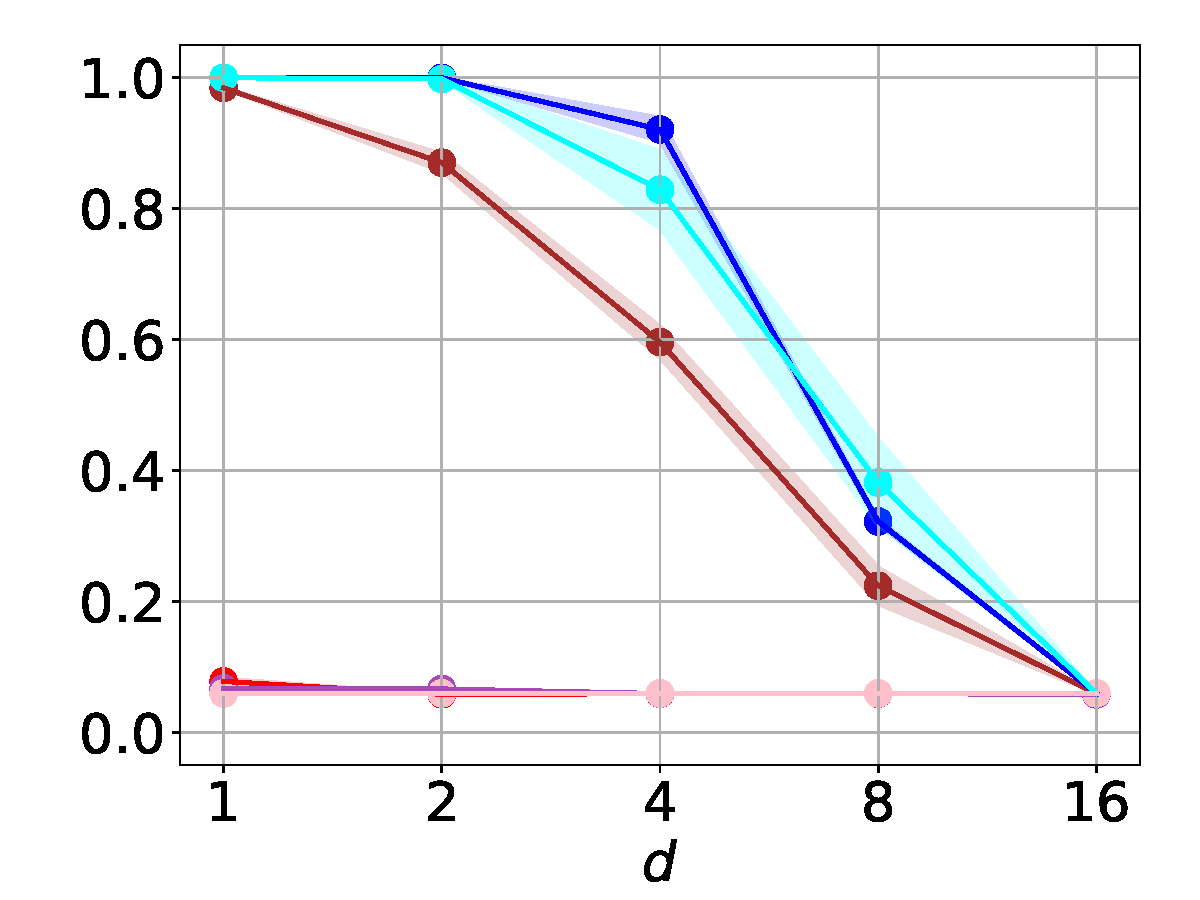
\includegraphics[width=\linewidth]{figs/long_range/fig(10, 10)/(32, d)Best_Test $F_1$.pdf}
        \caption{$(\ell=32, d)$}
        \label{fig:sub_long_range_(32,d)}
    \end{subfigure}
    \caption{Performance varying spatial and temporal distances in the long-range spatio-temporal tasks.}
    \label{fig:plots_long_range}
\end{figure*}
